\documentclass[reprint,english,notitlepage]{revtex4-1}
% if you want a single-column, remove reprint

% allows special characters (including æøå)
\usepackage[utf8]{inputenc}
\usepackage [norsk]{babel} %if you write norwegian
%\usepackage[english]{babel}  %if you write english


\usepackage{physics,amssymb}  % mathematical symbols (physics imports amsmath)
\usepackage{graphicx}         % include graphics such as plots
\usepackage{xcolor}           % set colors
\usepackage{hyperref}         % automagic cross-referencing (this is GODLIKE)
\usepackage{tikz}             % draw figures manually
\usepackage{listings}         % display code
\usepackage{subfigure}        % imports a lot of cool and useful figure commands
\usepackage{float}			  % force placement of tables and figures
\usepackage{minted}

\hypersetup{ % this is just my personal choice, feel free to change things
	colorlinks,
	linkcolor={red!50!black},
	citecolor={blue!50!black},
	urlcolor={blue!80!black}}

%% Defines the style of the programming listing
%% This is actually my personal template, go ahead and change stuff if you want
\lstset{ %
	inputpath=,
	backgroundcolor=\color{white!88!black},
	basicstyle={\ttfamily\scriptsize},
	commentstyle=\color{magenta},
	language=Python,
	morekeywords={True,False},
	tabsize=4,
	stringstyle=\color{green!55!black},
	frame=single,
	keywordstyle=\color{blue},
	showstringspaces=false,
	columns=fullflexible,
	keepspaces=true}

\begin{document}
	
\title{FYS4150 - Prosjekt 2}
\date{\today}               
\author{Karl Henrik Fredly}
\affiliation{Universitetet i Oslo} 

\newpage
	
\begin{abstract} %------------------Abstract-----------------------
	Hva skjer
	
	- Github repository link med all kode og resultater med ekstra forklaringer: \href{https://github.com/KarlHenrik/ComputationalPhysicsMaster/tree/master/FYS4150\%20-\%20Computational\%20Physics/Project\%202}{https://github.com/KarlHenrik/ComputationalPhysicsMaster/tree/master/FYS4150\%20-\%20Computational\%20Physics/Project\%202}
\end{abstract}
\maketitle

\section{Introduksjon} %------------------Introduksjon-----------------------
	Løsningen av den en-dimensjonale Poisson ligningen med Dirichlet grensebetingelser er en god øvelse i å jobbe med matriser, minneallokasjon, vektorer og å evaluere ulike løsningsmetoder.
	
	I metode seksjonen vil vi presentere problemet og utlede den generelle Thomas algoritmen og en versjon spesielt tilpasset problemet vi ser på. Vi vil også nemne LU faktorisering som en løsningsmetode.
	
	I resultat seksjonen presenterer vi løsningen av ligningen, hastigheten til metodene og hvordan feilen endrer seg med steglengde.
	
	Til dette prosjektet har jeg skrevet kode som implementerer den generelle Thomas algoritmen, og den spesielt tilpassede versjonen \cite{myRepo}. Jeg har også skrevet kode for å bearbeide og presentere resultatene fra denne koden \cite{myRepo}. For å løse ligningssettet med LU faktorisering brukte jeg ferdigskrevet kode fra kursets github repository \cite{libRepo}\cite{cspRepo}.


\section{Metoder} %------------------Metoder-----------------------
	Vi skal numerisk løse den en-dimensjonale Poisson ligningen med Dirichlet grensebetingelser.

\subsection{Ligningen vi skal løse}

	Vi begynner med å se på den tredimensjonale Poisson ligningen:
	
	\begin{equation*}
	\nabla^2 \Phi = -4\pi \rho (\mathbf{r}).
	\end{equation*}
	
	Krever vi sfærisk symmetrisk $\Phi$ og $\mathbf{r}$ forenkles dette til en en-dimensjonell ligning i r:
	
	\begin{equation*}
	\frac{1}{r^2}\frac{d}{dr}\left(r^2\frac{d\Phi}{dr}\right) = -4\pi \rho(r),
	\end{equation*}
	
	Vi substituerer $\Phi(r)= \phi(r)/r$ og får:
	
	\begin{equation*}
	\frac{d^2\phi}{dr^2}= -4\pi r\rho(r).
	\end{equation*}
	
	Definerer et kildeledd $f$ gitt ved ladningsfordelingen $\rho$ ganget med $r$ og konstanten $-4\pi$.
	
	Substituerer til slutt $\phi\rightarrow u$ og $r\rightarrow x$ og får ligningen vi skal løse i dette prosjektet:
	
	\begin{equation*}
	-u''(x) = f(x)
	\end{equation*}
	
	Vi løser denne med Dirichlet grensebetingelser som vil si at vi får ligningen med betingelser:
	
	\begin{equation*}
	-u''(x) = f(x), \hspace{0.5cm} x\in(0,1), \hspace{0.5cm} u(0) = u(1) = 0.
	\end{equation*}
	
	I vårt tilfelle bruker vi et kildledd gitt ved $f(x) = 100e^{-10x}$. Den analytiske løsningen blir da $u(x) = 1 - (1 - e^{-10})x - e^{-10x}$. Vi bruker denne til å måle feilen til den numeriske løsningen vår. (utregning tatt fra oppgavetekst \cite{oppgavetekst})

\subsection{Diskret tilnærming}

	Vi skal tilnærme $u(x)$ ved å regne ut verdiene $v_i$ i punktene $x_i = ih$. $x_i$ går fra $x_0 = 0$ til $x_{n+1} = 1$ med steglengde $h=1/(n+1)$. Vi har $v_0 = v_{n+1} = 0$. Vi tilnærmer den andrederiverte av $u$ med:
	
	\begin{equation*}
	\begin{aligned}
	-\frac{v_{i+1}+v_{i-1}-2v_i}{h^2} &= f_i  \hspace{0.5cm} \mathrm{for} \hspace{0.1cm} i=1,\dots, n \\
	-v_{i+1} - v_{i-1} + 2v_i &= f_i h^2 \\
	-v_{i+1} - v_{i-1} + 2v_i &= b_i
	\end{aligned}
	\end{equation*}
	hvor $f_i=f(x_i)$ og $b_i = f_i h^2$.
	
	Dette gir oss n ligninger som svarer til av $b_i$-ene fra n=1 til n. Siden $v_0 = v_{n+1} = 0$ forsvinner $v_{i-1}$ leddet i den første ligningen, og $v_{i+1}$ leddet i den siste ligningen. Vi kan skrive disse som
	
	\begin{equation*}
	\begin{aligned}
	\mathbf{A}\mathbf{v} = \tilde{\mathbf{b}}
	\end{aligned}
	\end{equation*}
	hvor

	\begin{equation*}
	\begin{aligned}
	\mathbf{A} = \begin{bmatrix}
	2& -1& 0 &\dots   & \dots &0 \\
	-1 & 2 & -1 &0 &\dots &\dots \\
	0&-1 &2 & -1 & 0 & \dots \\
	& \dots   & \dots &\dots   &\dots & \dots \\
	0&\dots   &  &-1 &2& -1 \\
	0&\dots    &  & 0  &-1 & 2 \\
	\end{bmatrix}
	\end{aligned}
	\end{equation*}
	og 
	\begin{equation*}
	\begin{aligned}
	\mathbf{v} = \begin{bmatrix}
	v_1 \\
	v_2 \\
	v_3 \\
	\dots \\
	v_{n-1} \\
	v_{n}
	\end{bmatrix},
	\tilde{\mathbf{b}} = \begin{bmatrix}
	\tilde{b}_1 \\
	\tilde{b}_2 \\
	\tilde{b}_3 \\
	\dots \\
	\tilde{b}_{n-1} \\
	\tilde{b}_{n}
	\end{bmatrix}
	\end{aligned}
	\end{equation*}

\subsection{Metode 1: Den generelle Thomas algoritmen}
	Matrisen $\mathbf{A}$ er en tridiagonal matrise, siden den kun har elementer på, rett over og rett under diagonalen. Generelt kan en tridiagonal matrise skrives som:
	
	\begin{equation*}
	\begin{aligned}
	\mathbf{A} = \begin{bmatrix}
	d_1 & c_1 & 0 &\dots   & \dots &0 \\
	a_1 & d_2 & c_2 &0 &\dots &\dots \\
	0& a_2 & d_3 & c_3 & 0 & \dots \\
	& \dots   & \dots &\dots   &\dots & \dots \\
	0&\dots   &  &a_{n-2} & d_{n-1} & c_{n-1} \\
	0&\dots    &  & 0  &a_{n-1} & d_n \\
	\end{bmatrix}
	\end{aligned}
	\end{equation*}
	
	Vi kan løse ligningen $\mathbf{A}\mathbf{v} = \tilde{\mathbf{b}}$ med denne generelle tridiagonale matrisen $\mathbf{A}$ med Thomas algoritmen. Først eliminerer man $a_i$-ene med forlengssubstitusjon, og så løser man ligningssystemet med baklengssubstitusjon.
	
	For forlengssubstitusjon ser vi at vi ikke trenger å endre på første rad. På andre rad trekker vi fra første rad ganget med $a_1/d_1$, for å eliminere $a_1$. Da får vi et nytt diagonalelement $\tilde{d}_2 = d_2 - c_1 * a_1/d_1$ og et nytt element på høyresiden $b_2 = \tilde{b}_2 - \tilde{b}_1 * a_1/d_1$.
	
	Når vi videre skal eliminere $a_2$ på tredje rad ser vi at vi har samme situasjon som vi hadde i andre rad, bare forskjøvet et hakk til høyre. Og alle stegene videre vil være helt like. Vi får formlene:
	
	\begin{equation*}
	\begin{aligned}
	\tilde{d}_i = d_i - c_{i-1} * a_{i-1}/d_{i-1} \hspace{0.4cm} og \hspace{0.4cm} b_i = \tilde{b}_i - \tilde{b}_{i-1} * a_{i-1}/d_{i-1}
	\end{aligned}
	\end{equation*}
	for $i=2,\dots, n$.
	
	Når vi gjør baklengssubstitusjonen finner vi verdiene $v_i$ ved å bevege oss baklengs gjennom matrisen. Siste rad vil kun inneholde $\tilde{d}_n$, siden $a_n$ ble eliminert. Vi setter derfor $v_n = b_n / \tilde{d}_n$. Ved ant siste rad har vi kun igjen $\tilde{d}_{n-1}$ og $c_{n-1}$, men nå vet vi $v_n$, så vi finner $v_{n-1} = (b_{n-1} - c_{n-1}v_{n}) / \tilde{d}_{n-1}$. Ved tredje siste rad og videre har vi samme situasjon og vi får:
	
	\begin{equation*}
	\begin{aligned}
	v_{i} = (b_{i} - c_{i}v_{i+1}) / \tilde{d}_{i}
	\end{aligned}
	\end{equation*}
	for $i=n-1,\dots, 1$.
	
	Etter dette har vi funnet alle punktene $v_i$ vi var ute etter. For hvert steg har vi tre induktive formler med til sammen 9 FLOPs. Metoden bruker dermed 9n FLOPs, og er i størrelsesorden $\order{n}$ (kan reduseres til 8n FLOPs ved å regne ut $a_{i-1}/d_{i-1}$ kun en gang for hvert steg).
	
	Metoden er implementert i filen tridiagSlow.cpp, som finnes i det vedlagte github repositoriet \cite{myRepo}. Et relevant kodeutsnitt som viser forlengs- og baklengssubstitusjonen er vist her:
	
	\begin{minted}[mathescape, linenos]{python}
double factor;
for (int i = 2; i < n; i++) {
    factor = a[i - 1] / d[i - 1];
    d[i] = d[i] - c[i - 1] * factor;
    b[i] = b[i] - b[i - 1] * factor;
}
sol[n-1] = b[n-1] / d[n-1];
for (int i = n - 2; i > 0; i--) {
    sol[i] = (b[i] - c[i] * sol[i + 1]) / d[i];
}
	\end{minted}

\subsection{Metode 2: Vårt spesialtilfelle}

	I vårt tilfelle vet vi alle elementene i A, og langs diagonalene er de radvis like. Den første konsekvensen av dette er at vi kan regne ut oppdateringen av hovuddiagonalen på forhånd (slik at de ikke regnes med i antall FLOPs). Formelen:
	
	\begin{equation*}
	\begin{aligned}
	\tilde{d}_i &= d_i - c_{i-1} * a_{i-1}/d_{i-1} \\
	&= d_i - (-1) * (-1)/d_{i-1} \\
	&= d_i - 1/d_{i-1}
	\end{aligned}
	\end{equation*}
	for $i=2,\dots, n$, med $d_1 = 2$ gir $d_i = \frac{i + 1}{i}$ for $i=1,\dots, n$.
	
	Forlengssubstitusjonen blir:
	
	\begin{equation*}
	\begin{aligned}
	b_i &= \tilde{b}_i - \tilde{b}_{i-1} * a_{i-1}/d_{i-1} \\
	&= \tilde{b}_i - \tilde{b}_{i-1} * (-1)/d_{i-1} \\
	&= \tilde{b}_i + \tilde{b}_{i-1} /d_{i-1}
	\end{aligned}
	\end{equation*}
	for $i=2,\dots, n$.
	
	Og baklengssubstitusjonen blir:
	
	\begin{equation*}
	\begin{aligned}
	v_{i} &= (b_{i} - c_{i}v_{i+1}) / \tilde{d}_{i} \\
	&= (b_{i} - (-1)v_{i+1}) / \tilde{d}_{i} \\
	&= (b_{i} + v_{i+1}) / \tilde{d}_{i}
	\end{aligned}
	\end{equation*}
	for $i=n-1,\dots, 1$.
	
	For hvert steg har vi da 4 FLOPs, så metoden bruker til sammen 4n flops som er i størrelsesorden $\order{n}$.
	
	Metoden er implementert i filen tridiag.cpp, som finnes i det vedlagte github repositoriet \cite{myRepo}. Et relevant kodeutsnitt som viser forlengs- og baklengssubstitusjonen er vist her:
	
	\begin{minted}[mathescape, linenos]{python}
for (int i = 2; i < n; i++) {
    b[i] = b[i] + b[i - 1] / d[i - 1];
}
sol[n-1] = b[n-1] / d[n-1];
for (int i = n - 2; i > 0; i--) {
    sol[i] = (b[i] + sol[i + 1]) / d[i];
}
	\end{minted}
	
	
\subsection{Metode 3: LU faktorisering og løsing}
	LU faktorisering er en kjent metode som kan brukes til å løse ligningssett på formen $\mathbf{A}\mathbf{v} = \tilde{\mathbf{b}}$, som går ut på å faktorisere $\mathbf{A}$ inn i en nedre triangulær matrise $\mathbf{L}$ og en øvre triangulær matrise $\mathbf{U}$, for så å enkelt løse ligningene $\mathbf{A}\mathbf{y} = \tilde{\mathbf{b}}$ og $\mathbf{U}\mathbf{v} = \mathbf{y}$ \cite{luwiki}.
	
	LU faktorisering tar omtrent $\frac{2}{3}n^3$ FLOPs, og er dermed på størrelsesorden $\order{n^3}$.
	
	Metoden er brukt i programmet tridiagLU.cpp, som finnes i det vedlagte github repositoriet\cite{myRepo}. Jeg importerer funksjoner fra filen lib.cpp, tatt fra githubsiden til kurset\cite{libRepo}, for å løse ligningssettet med LU faktorisering.
	
	For å sammenligne hastigheten til metodene importerer jeg ''time.h'' i C++, og bruker funksjonen clock(). Tidtakingen blir gjort i programmet ''tridiagTiming.cpp''.

\section{Resultater} %------------------Resultater-----------------------
	Alle tre metodene gir samme funksjonsverdier for n opp til 1000. Testet kun verdiene til den tilpassede Thomas algoritmen for høyere n enn det. Viser ikke tabeller av verdier her for å vise det, men resultatene ligger med koden på github\cite{myRepo}.
	
	Programmet ''tridiagSlow.cpp'' bruker den generelle Thomas algoritmen til å løse ligningen. Kjørte programmet for n = 10 punkter, og får plottet i figur \ref{fig:losning1} med notebooken ''Project1Notebook.ipynb'' \cite{myRepo}.

	\begin{figure}[H]
		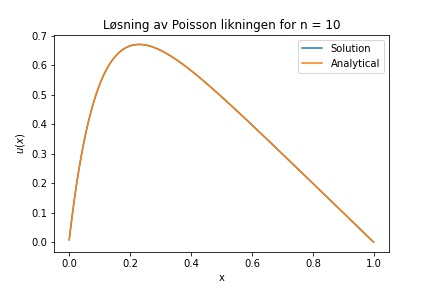
\includegraphics[width=90mm]{../Results/losning1.jpg}
		\caption{Analytisk og numerisk løsning av 1d Poisson ligningen. Brukte her den tilpassede Thomas algoritmen.}
		\label{fig:losning1}
	\end{figure}

	Kjørte tilsvarende programmet ''tridiag.cpp'' som bruker den tilpassede versjonen av Thomas algoritmen for n = 1000 punkter og får plottet i figur \ref{fig:losning} med samme notebook.

	\begin{figure}[H]
		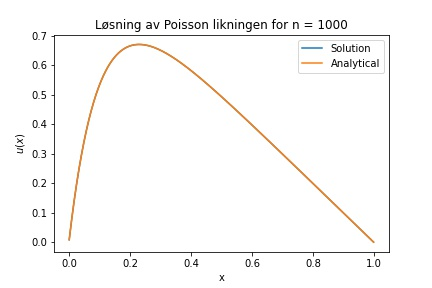
\includegraphics[width=90mm]{../Results/losning.jpg}
		\caption{Analytisk og numerisk løsning av 1d Poisson ligningen. Brukte her den tilpassede Thomas algoritmen.}
		\label{fig:losning}
	\end{figure}
	
	Kjørte programmet ''tridiag.cpp'' som bruker den tilpassede versjonen av Thomas algoritmen for n = 1000 punkter og får plottet i figur \ref{fig:relErr3}. Den viser hvordan den relative feilen endrer seg fra punkt til punkt for liten n. Figur \ref{fig:relErr7} produsert på tilsvarende vis med n = $10^7$ viser hvordan feilen endrer seg fra punkt til punkt for stor n.
	
	\begin{figure}[H]
		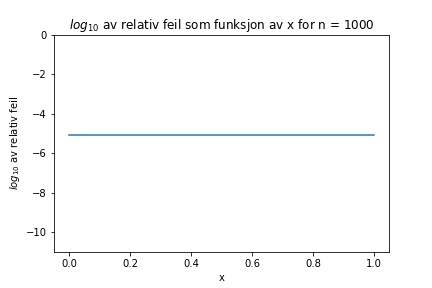
\includegraphics[width=90mm]{../Results/relErrx.jpg}
		\caption{$log_{10}$ av relativ feil for alle punktene for n = 1000.}
		\label{fig:relErr3}
	\end{figure}

	\begin{figure}[H]
		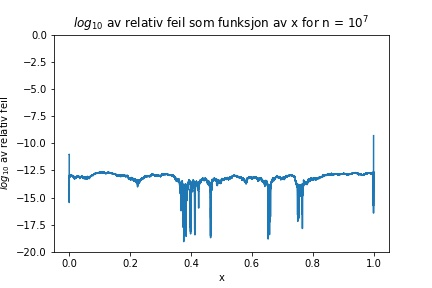
\includegraphics[width=90mm]{../Results/relErr7.jpg}
		\caption{$log_{10}$ av relativ feil for alle punktene for n = $10^7$.}
		\label{fig:relErr7}
	\end{figure}

	Tiden de ulike metodene brukte på å løse ligningen for ulike n vises i tabell \ref{tab:tid}. 
	
	\begin{table}[H]
		\begin{center}
			\caption{Tid for de ulike metodene i sekunder.}
			\label{tab:tid}
			\begin{tabular}{|c|c|c|c|} \hline
				\textbf{$log_{10}(n)$} & \textbf{Tridiag} & \textbf{Tridiag Generell} & \textbf{LU} \\ \hline
				1 & 0.00000 & 0.00000 & 0.00000 \\
				2 & 0.00000 & 0.00000 & 0.00100 \\
				3 & 0.00000 & 0.00000 & 1.17000 \\
				4 & 0.00000 & 0.00000 & 2228.8350 \\
				5 & 0.00200 & 0.00200 & \\
				6 & 0.01400 & 0.01800 & \\
				7 & 0.13600 & 0.17700 & \\ \hline
			\end{tabular}
		\end{center}
	\end{table}
	Tabell \ref{tab:flops} viser omtrent hvor mange FLOPs hver metode bruker for ulike n.
	\begin{table}[H]
		\begin{center}
			\caption{FLOPs for de ulike metodene.}
			\label{tab:flops}
			\begin{tabular}{|c|c|c|c|} \hline
				\textbf{$log_{10}(n)$} & \textbf{Tridiag (4n)} & \textbf{Tridiag Generell(8n)} & \textbf{LU(2/3$n^3$)} \\ \hline
				1 & 4$*10$ & 8$*10$ & $6.67*10^{2}$ \\
				2 & 4$*10^2$ & 8$*10^{2}$ & $6.67*10^{5}$ \\
				3 & 4$*10^3$ & 8$*10^{3}$ & $6.67*10^{8}$ \\
				4 & 4$*10^4$ & 8$*10^{4}$ & $6.67*10^{11}$ \\
				5 & 4$*10^5$ & 8$*10^{5}$ & $6.67*10^{14}$\\
				6 & 4$*10^6$ & 8$*10^{6}$ & $6.67*10^{17}$\\
				7 & 4$*10^7$ & 8$*10^{7}$ & $6.67*10^{20}$\\ \hline
			\end{tabular}
		\end{center}
	\end{table}

	Endringen av relativ feil som funksjon av økende n vises i tabell \ref{tab:relErr} og i figur \ref{fig:relErrPlot}. Vi ser her på den største enkeltfeilen mellom analytisk og numerisk løsning. For n = $10^6$ er feilen litt under -11 for alle punktene borsett fra de ved endepunktene.
	
	\begin{table}[H]
		\begin{center}
			\caption{$log_{10}$ av relativ feil som funksjon av $log_{10}(n)$}
			\label{tab:relErr}
			\begin{tabular}{|c|c|} \hline
				\textbf{$log_{10}(n)$} & $log_{10}(|\frac{v_i - u_i}{u_i}|)$ \\ \hline
				1 & -1.1005822 \\
				2 & -3.070673 \\
				3 & -5.079183 \\
				4 & -7.079094 \\
				5 & -9.079008 \\
				6 & -10.431693 \\
				7 & -9.2979409 \\ \hline
			\end{tabular}
		\end{center}
	\end{table}
	
	\begin{figure}[H]
		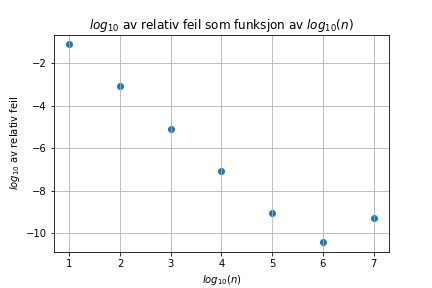
\includegraphics[width=90mm]{../Results/relErrPlot.jpg}
		\caption{$log_{10}$ av relativ feil som funksjon av $log_{10}(n)$.}
		\label{fig:relErrPlot}
	\end{figure}
	
\section{Diskusjon} %------------------Diskusjon-----------------------
	Vi observerte at alle tre metodene finner samme funksjonsverdier for n = 10 opp til 1000 (testet ikke tallene til alle metodene for større n). Dette skyldes trolig at alle metodene manipulerer matriseelementer til å finne en ''eksakt'' løsning til det samme ligningssettet.
	
	På figur \ref{fig:losning} ser vi at den numeriske og analytiske løsningen passer godt sammen, og i tabell \ref{tab:relErr} ser vi at de passer bedre og bedre sammen for større n helt til rundt n = $10^6$, da den øker litt. Dette ser vi også på figur \ref{fig:relErrPlot}, hvor et stigningstall på ca. -2 er tydelig for de fem første punktene(dette kommer av mindre avkortingsfeil gitt mindre h). Hvis vi hadde sett på gjennomsnittlig feil, hadde også det sjette punktet vært på denne linjen. Ved n = $10^7$ mister vi nøyaktighet fordi tallene vi regner med er for små til å holde på nyttig informasjon, vi ser at dette fører til variasjon i verdiene vi får ut i figur \ref{fig:relErr7}, sammenlignet med figur \ref{fig:relErr3}. Vi får derfor her best resultat for n = $10^6$.
	
	Vi fikk tatt tiden på de to versjonene av Thomas algoritmen opp til n = $10^7$, da den generelle versjonen brukte 0.177s og den tilpassede versjonen brukte 0.136s. Som vi ser i tabell \ref{tab:flops} skal den tilpassede versjonen utføre halvparten så mange FLOPs, men vi ser at den allikevel ikke er dobbelt så rask. Dette skyldes trolig tiden det tar å lese og skrive til minnet, samt andre ukontrollerbare effekter. Høyere n hadde vi ikke minnekapasitet til å regne ut for. LU metoden gjør betydelig flere FLOPs, som man ser i tabell \ref{tab:flops}, og den bruker naturligvis mye lengre tid. Fra n = 1000 til n = 10000 brukte den rundt 2000 ganger lengre tid, selv om det kun var 1000 ganger flere FLOPs, dette skyldes trolig den store mengden data som må lagres, skrives og leses siden vi bruker nxn matriser. For n = 10000 brukte LU metoden litt over 37 minutter. Ganger vi det med kun 1000 (siden det blir 1000 ganger flere FLOPs for n = $10^5$), får vi litt under 26 dager, så vi kan slå fast at LU metoden fungerer særs dårlig til å løse dette problemet.


\section{Konklusjon} %------------------Konklusjon-----------------------
	Vi løste den en-dimensjonale Poisson ligningen med Dirichlet grensebetingelser numerisk. Vi implementerte tre ulike metoder for å løse ligningen, og sammenlignt kompleksiteten og hastigheten til disse. LU faktorisering har en kompleksitet på $2/3n^3$, og brukte dermed lang tid på å løse ligningen med kort steglengde. Den generelle Thomas algoritmen har en kompleksitet på $8n$ og var dermed effektiv også for små steglengder. Den tilpassede Thomas algoritmen har en kompleksitet på $4n$ og presterte best av alle metodene. Det er tydelig at valg av metode kan ha mye å si for hvor effektivt man kan løse et problem, siden LU faktorisering brukte 37 minutter på å regne ut noe de andre metodene gjorde nærmest umiddelbart.

\begin{figure*} \bibliography{biblio} \end{figure*}
	
\end{document}